
\medskip 

\parbox{0.43\linewidth}{On considère le programme de calcul ci-contre dans lequel x, Étape 1,
Étape 2 et 

Résultat sont quatre variables.}\hfill
\parbox{0.53\linewidth}{{
%\begin{tabular}{|l|}\hline
%\textbf{Créer une variable}\\
%Étape 1\\
%Étape 1\\
%Résultat\\
%x\\ \hline
%\end{tabular}

\includegraphics[width=3cm]{VariablesPondichery2017.eps}

%\textbf{Programme Scratch}

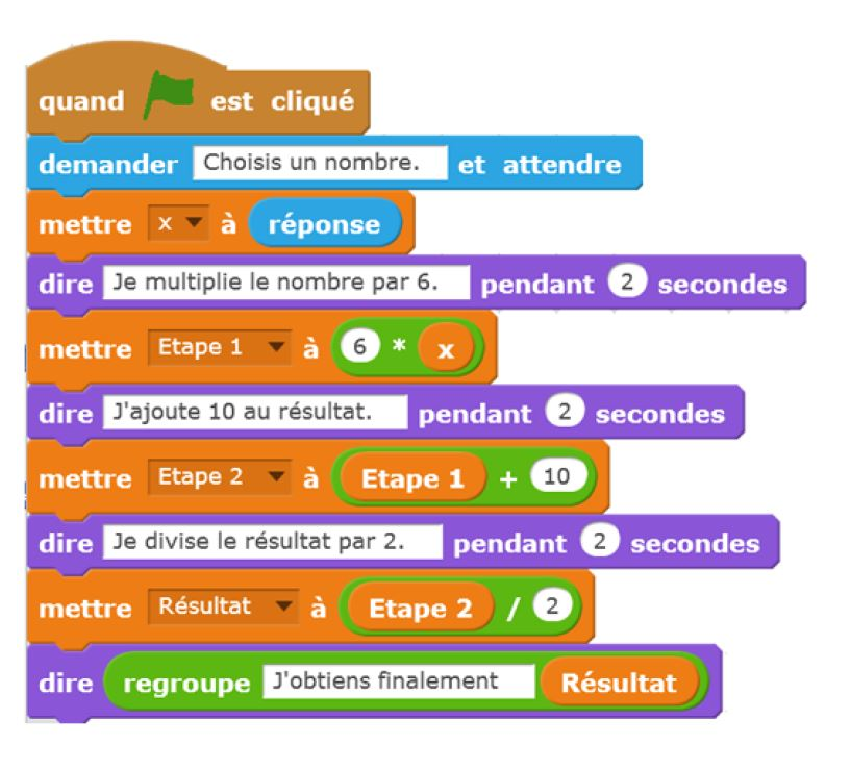
\includegraphics[width=7cm]{Pondichery2017.eps}
%\begin{tabular}{|l|}\hline
%quand le drapeau est cliqué\\
%demander Choisis un nombre et attendre\\mettre x à réponse\\
%dire Je multiplie le nombre par 6 pendant 2 secondes\\
%mettre Étape 1  à 6 * x\\
%dire J'ajoute 10 au résultat pendant 2 secondes\\
%mettre Étape 2 à Étape 1 + 10\\
%dire Je divise le résultat par 2 pendant 2 secondes\\
%mettre Résultat à Étape 2 / 2\\
%dire regroupe J'obtiens finalement Résultat\\ \hline
%\end{tabular}
}}

\medskip

\begin{enumerate}
\item 
	\begin{enumerate}
		\item Julie a fait fonctionner ce programme en choisissant le nombre 5. Vérifier que
ce qui est dit à la fin est: \og J'obtiens finalement 20 \fg.
		\item Que dit le programme si Julie le fait fonctionner
en choisissant au départ le nombre 7 ?
	\end{enumerate}
\item Julie fait fonctionner le programme, et ce qui est dit à
la fin est: \og J'obtiens finalement 8 \fg.
Quel nombre Julie a-t-elle choisi au départ ?
\item Si l'on appelle x le nombre choisi au départ, écrire en
fonction de x l' expression obtenue à la fin du programme, puis réduire cette expression autant que
possible.
\item Maxime utilise le programme de calcul ci-dessous :
\begin{center}	
\begin{tabularx}{0.5\linewidth}{|l X|}\hline
$\bullet~~$&Choisir un nombre.\\
$\bullet~~$&Lui ajouter 2\\
$\bullet~~$&Multiplier le résultat par 5\\\hline
\end{tabularx}
\end{center}

Peut-on choisir un nombre pour lequel le résultat obtenu par Maxime est le même que celui obtenu par
Julie ?	
\end{enumerate}

\bigskip
 
